\documentclass[journal]{IEEEtran}
\usepackage[a5paper, margin=10mm, onecolumn]{geometry}
\usepackage{lmodern}
\usepackage{tfrupee}
\setlength{\headheight}{1cm} % Set the height of the header box
\setlength{\headsep}{0mm}  % Set the distance between the header box and the top of the text

\usepackage{csquotes}
\usepackage{gvv-book}
\usepackage{gvv}
\usepackage{circuitikz}
\usepackage{cite}
\usepackage{amsmath,amssymb,amsfonts,amsthm}
\usepackage{algorithmic}
\usepackage{graphicx}
\usepackage{textcomp}
\usepackage{xcolor}
\usepackage{txfonts}
\usepackage{listings}
\usepackage{enumitem}
\usepackage{mathtools}
\usepackage{gensymb}
\usepackage{comment}
\usepackage[breaklinks=true]{hyperref}
\usepackage{tkz-euclide} 
\usepackage{listings}
% \usepackage{gvv}                                        
\def\inputGnumericTable{}                                 
\usepackage[latin1]{inputenc}                                
\usepackage{color}                                            
\usepackage{array}                                            
\usepackage{longtable}                                       
\usepackage{calc}                                             
\usepackage{multirow}                                         
\usepackage{hhline}                                           
\usepackage{ifthen}                                           
\usepackage{lscape}
\usepackage{caption}
\usepackage{tikz}
\usetikzlibrary{patterns}
\begin{document}

\bibliographystyle{IEEEtran}


\begin{center}
    \textbf{\Large GATE 2024\\
    AGRICULTURAL ENGINEERING (AG)\\
    MAIN PAPER}
\end{center}

\section*{General Aptitude (GA)}
\subsection*{Q.1 -- Q.5 Carry ONE mark Each}

\begin{enumerate}
 \item
If '$\rightarrow$' denotes increasing order of intensity, then the meaning of the words\\
$[$dry $\rightarrow$ arid $\rightarrow$ parched$]$ is analogous to $[$diet $\rightarrow$ fast $\rightarrow$ \dots $]$.\\
 Which one of the given options is appropriate to fill the blank?
    
 \begin{enumerate}
 \begin{multicols}{2}
        \item starve
        \item reject
        \item feast
        \item deny
    \end{multicols}
    \end{enumerate}
    \hfill(GATE AG 2024)\\

    \medskip

\item
If two distinct non-zero real variables $x$ and $y$ are such that $(x+y)$ is proportional to $(x-y)$ then the value of $\frac{x}{y}$ is
    \begin{enumerate}
    \begin{multicols}{2}
        \item depends on $xy$
        \item depends only on $x$ and not on $y$
        \item depends only on $y$ and not on $x$
        \item is a constant
    \end{multicols}
    \end{enumerate}
     \hfill(GATE AG 2024)\\

 \medskip


\item 
Consider the following sample of numbers:

\[
9,\ 18,\ 11,\ 14,\ 15,\ 17,\ 10,\ 69,\ 11,\ 13
\]

The median of the sample is

\begin{enumerate}
\begin{multicols}{2}
    \item 13.5
    \item 14
    \item 11
    \item 18.7
\end{multicols}
\end{enumerate}
 \hfill(GATE AG 2024)\\

 \medskip

\item 
The number of coins of $\rupee1$, $\rupee5$, and $\rupee10$ denominations that a person has are in the ratio $5:3:13$. Of the total amount, the percentage of money in $\rupee5$ coins is

\begin{enumerate}
\begin{multicols}{2}
    \item 21\%
    \item $14 \frac{2}{7}\%$
    \item 10\%
    \item 30\%
\end{multicols}
\end{enumerate}
 \hfill(GATE AG 2024)\\

 \medskip

\item
For positive non-zero real variables $p$ and $q$, if
\begin{equation*}
    \log \left( p^2 + q^2 \right) = \log p + \log q + 2\log 3,
\end{equation*}
then, the value of\quad 
\[
\frac{p^4 + q^4}{p^2 q^2}
\]
is
\begin{enumerate}
\begin{multicols}{2}
    \item 79
    \item 81
    \item 9
    \item 83
\end{multicols}
\end{enumerate}
 \hfill(GATE AG 2024)\\

\medskip

\noindent
Q.6\quad -- Q.10 Carry TWO marks Each

\item 
In the given text, the blanks are numbered (i)--(iv). Select the best match for all the blanks.\\

Steve was advised to keep his head \dots (i) before heading \dots (ii) to bat; for, while he had a head \dots (iii) batting, he could only do so with a cool head \dots (iv) his shoulders.

\begin{enumerate}
\begin{multicols}{2}
    \item (i) down \quad (ii) down \quad (iii) on \quad (iv) for
    \item (i) on \quad (ii) down \quad (iii) for \quad (iv) on
    \item (i) down \quad (ii) out \quad (iii) for \quad (iv) on
    \item (i) on \quad (ii) out \quad (iii) on \quad (iv) for
\end{multicols}
\end{enumerate}
 \hfill(GATE AG 2024)\\

 \medskip

\item 
A rectangular paper sheet of dimensions $54~\text{cm} \times 4~\text{cm}$ is taken. The two longer edges of the sheet are joined together to create a cylindrical tube. A cube whose surface area is equal to the area of the sheet is also taken.

Then, the ratio of the volume of the cylindrical tube to the volume of the cube is

\begin{enumerate}
\begin{multicols}{2}
    \item $\frac{1}{\pi}$
    \item $\frac{2}{\pi}$
    \item $\frac{3}{\pi}$
    \item $\frac{4}{\pi}$
\end{multicols}
\end{enumerate}
 \hfill(GATE AG 2024)\\

 \medskip

\item 
The pie chart presents the percentage contribution of different macronutrients to a typical 2,000 kcal diet of a person.

\medskip

\begin{figure}[h]
    \centering
    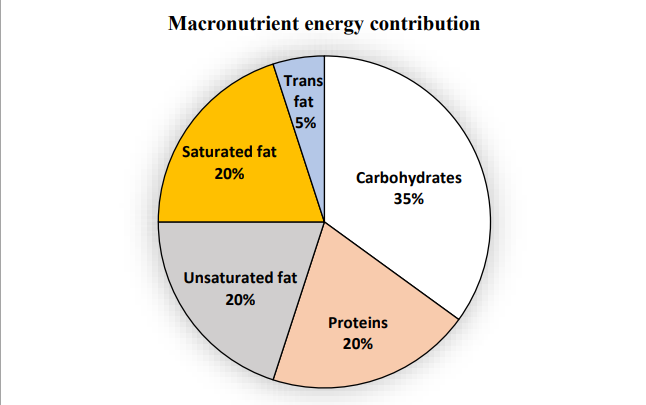
\includegraphics[width=0.7\columnwidth]{Figs/Screenshot 2025-08-24 210825.png}
    \caption{}
    \label{fig 1}
\end{figure}

\medskip

The typical energy density (kcal/g) of these macronutrients is given in the table.

\begin{tabular}{>{\bfseries}l l}
Specification & Outer Diameter in mm \\
P. AW & p. 34.9 \\
Q. BW & q. 44.4 \\
R. EW & r. 54.0 \\
S. NW & s. 66.7 \\
\end{tabular}



\medskip

The total fat (all three types), in grams, this person consumes is
\begin{enumerate}
\begin{multicols}{2}
  \item 44.4
  \item 77.8
  \item 100
  \item 3,600
\end{multicols}
\end{enumerate}
 \hfill(GATE AG 2024)\\

 \medskip

\item 
A rectangular paper of $20\,\mathrm{cm} \times 8\,\mathrm{cm}$ is folded $3$ times. Each fold is made along the line of symmetry, which is perpendicular to its long edge. The perimeter of the final folded sheet (in cm) is

\begin{enumerate}
\begin{multicols}{4}
\item  18
\item  24
\item  20  
\item  21
\end{multicols}
\end{enumerate}
 \hfill(GATE AG 2024)\\

\medskip

\item 
The least number of squares to be added in the figure to make AB a line of symmetry is

\begin{figure}[h]
    \centering
    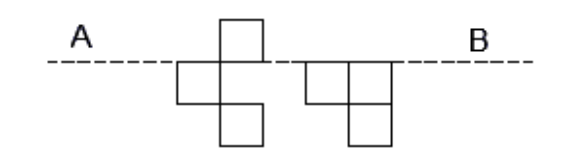
\includegraphics[width=0.7\columnwidth]{Figs/Screenshot 2025-08-24 211142.png}
    \caption{}
    \label{fig 1}
\end{figure}

\begin{enumerate}
\begin{multicols}{4}
\item 6   
\item 4
\item 5  
\item 7
\end{multicols}
\end{enumerate}
 \hfill(GATE AG 2024)\\

 \medskip

\section*{Q.11 - Q.35 Carry ONE mark Each}

\item
The divergence of the curl of a twice continuously differentiable vector function is \dots.
    \begin{enumerate}
    \begin{multicols}{2}
        \item 0
        \item 1
        \item 2
        \item $\infty$
    \end{multicols}
    \end{enumerate}
     \hfill(GATE AG 2024)\\

     \medskip

\item
Laplace transform of a function $f(t) = t^4$ as a function of '$s$' is \dots.
    \begin{enumerate}
    \begin{multicols}{2}
        \item $\frac{120}{s^5}$
        \item $\frac{24}{s^5}$
        \item $\frac{120}{s^4}$
        \item $\frac{24}{s^4}$
    \end{multicols}
    \end{enumerate}
     \hfill(GATE AG 2024)\\

 \medskip


\item
If the dynamic weight on the front axle is lesser than 20\% of the total weight of tractor, the longitudinal instability of tractor can be avoided by \dots.
    \begin{enumerate}
    \begin{multicols}{2}
        \item adding weight on the rear axle
        \item adding weight on the front axle
        \item reducing weight on the rear axle
        \item reducing weight on the front axle
    \end{multicols}
    \end{enumerate}
     \hfill(GATE AG 2024)\\

     \medskip

\item
In places with severe cold climate, the most important fuel property to be considered for running an internal combustion engine is \dots.
    \begin{enumerate}
    \begin{multicols}{2}
        \item heating value
        \item flash point
        \item pour point
        \item boiling point
    \end{multicols}
    \end{enumerate}
     \hfill(GATE AG 2024)\\

     \medskip


\item
A towed rigid wheel with a total weight $W$ is to be rolled on a hard horizontal surface as well as up the slope on a hard surface inclined at an angle $\theta$ with the horizontal. The rolling resistance of the wheel on inclined surface as compared to that on the horizontal surface is \dots.

\begin{enumerate}
\begin{multicols}{2}
  \item increased by $W\sin\theta$
  \item increased by $W\cos\theta$
  \item decreased by $W\sin\theta$
  \item decreased by $W\cos\theta$
\end{multicols}
\end{enumerate}
 \hfill(GATE AG 2024)\\

 \medskip

\item 
The difference between advance curve and recession curve for a given surface irrigation event is known as \dots.

\begin{enumerate}
\begin{multicols}{2}
  \item time of concentration
  \item lag time
  \item time to peak
  \item intake opportunity time
\end{multicols}
\end{enumerate}
 \hfill(GATE AG 2024)\\

 \medskip


\item 
Match the following instruments (in Column I) with corresponding measurements (in Column II).

\begin{center}
\begin{tabular}{|c|c|c|c|c|c|}
\hline
Mass of particles, g      & 2   & 5   & 7   & 4   & 1    \\
\hline
Mean size of particles, $\mu$m & 350 & 240 & 200 & 150 & 100 \\
\hline
\end{tabular}
\end{center}

\begin{enumerate}
\begin{multicols}{2}
  \item P-3,\quad Q-5,\quad R-4,\quad S-2,\quad T-1
  \item P-2,\quad Q-3,\quad R-5,\quad S-1,\quad T-4
  \item P-1,\quad Q-2,\quad R-3,\quad S-4,\quad T-5
  \item P-5,\quad Q-4,\quad R-1,\quad S-3,\quad T-2
\end{multicols}
\end{enumerate}
 \hfill(GATE AG 2024)\\

 \medskip

\item
In wind erosion, the maximum portion of soil is transported by the process of \dots.
    \begin{enumerate}
    \begin{multicols}{2}
        \item suspension
        \item saltation
        \item surface creep
        \item bed load
    \end{multicols}
    \end{enumerate}
     \hfill(GATE AG 2024)\\

     \medskip

\item 
 Hilly areas receiving heavy rainfall, where a major portion of the rainfall is to be drained as surface runoff, are suggested to adopt bench terraces with \dots.
    \begin{enumerate}
    \begin{multicols}{2}
        \item sloping inward
        \item level tops
        \item sloping outward
        \item narrow width
    \end{multicols}
    \end{enumerate}
     \hfill(GATE AG 2024)\\

     \medskip

\item
Critical thickness of insulation ($r_{cr}$) for a pipe having thermal conductivity (k) and convective heat transfer coefficient ($h_0$) is \dots.
    \begin{enumerate}
    \begin{multicols}{2}
        \item $2k/h_0$
        \item $k/h_0$
        \item $h_0/k$
        \item $2h_0/k$
    \end{multicols}
    \end{enumerate}
     \hfill(GATE AG 2024)\\

     \medskip

\item
A continuously differentiable function $y = f(x)$ satisfies one or more of the following conditions at its point of inflection:
    \begin{enumerate}
    \begin{multicols}{2}
      \item $\displaystyle \frac{d^2y}{dx^2} \neq 0$
      \item $\displaystyle \frac{d^2y}{dx^2} = 0$
      \item $\displaystyle \frac{d^3y}{dx^3} = 0$
      \item $\displaystyle \frac{d^3y}{dx^3} \neq 0$
    \end{multicols}
    \end{enumerate}
     \hfill(GATE AG 2024)\\

     \medskip

\item
In-situ volumetric soil moisture content measuring method(s) is/are:
    \begin{enumerate}
    \begin{multicols}{2}
      \item Neutron probe
      \item Tensiometer
      \item Time domain reflectometry
      \item Piezometer
    \end{multicols}
    \end{enumerate}
     \hfill(GATE AG 2024)\\

     \medskip

\item
Incorrect statement(s) with respect to hydrothermal treatment of paddy is/are:
    \begin{enumerate}
    \begin{multicols}{2}
      \item Process imparts hard texture to grain
      \item Retention of Vitamin B is less
      \item Cooking to the same degree of softness requires less time
      \item Bran obtained contains higher oil content
    \end{multicols}
    \end{enumerate}
     \hfill(GATE AG 2024)\\

     \medskip

\item
Falling rate period of drying can be explained by one/more of the following:
    \begin{enumerate}
    \begin{multicols}{2}
      \item Capillary rise of water
      \item Molecular diffusion of water
      \item Surface cooling
      \item Surface evaporation
    \end{multicols}
    \end{enumerate}
     \hfill(GATE AG 2024)\\

     \medskip

\item
The mean and variance of a dataset are 16 and 25, respectively. The coefficient of variation of the dataset, in \%, is \dots. \textit{(Rounded off to 2 decimal places)}
 \hfill(GATE AG 2024)\\

   \medskip
  
\item
The chances for passing an endurance test for three threshers P, Q and R are 1/6, 1/4, and 1/2, respectively. The probability of passing the endurance test by at least one thresher, in fraction, is \dots. \textit{(Rounded off to 2 decimal places)}
 \hfill(GATE AG 2024)\\

 \medskip

\item
The height of adult males at 5\textsuperscript{th}, 50\textsuperscript{th} and 95\textsuperscript{th} percentiles are 162 cm, 173 cm and 185 cm, respectively. The minimum inside height of the tractor cab required to ensure the satisfactory design based on the given data, in cm, is \dots.\\
(\textit{Answer in integer})
 \hfill(GATE AG 2024)\\

\medskip

\item
A chain drive is used to transmit power from a DC motor to the shaft of a solar energy operated thresher by reducing the speed from 240 rpm to 120 rpm. The number of teeth on the driving sprocket is 20 and the pitch circle diameter of the driven sprocket is 600 mm. The pitch of the chain used, in mm, is \dots.\\
(\textit{Rounded off to 2 decimal places})
 \hfill(GATE AG 2024)\\

\medskip

\item
A tractor drawn rotavator with a rotor radius 300 mm has 6 flanges having 3 blades in each flange acting in one plane. It is operated at a rotor speed of 180 rpm and a forward speed of 3 km$\cdot$h$^{-1}$. Increasing the forward speed as well as the rotor speed by 15\% each, the change in the length of soil slice, in mm, is \dots. (\textit{Answer in integer})
 \hfill(GATE AG 2024)\\

\medskip

\item
The air standard cycle efficiency of the Otto cycle is 56\% and heat supplied is 12.5 kJ, the heat rejected during the cycle, in kJ, is \dots.\\
(\textit{Rounded off to 2 decimal places})
 \hfill(GATE AG 2024)\\

\medskip

\item
The slope length of an area having land slope of 6\% is reduced to half while other conditions are kept unchanged. The reduction in annual soil loss from the area, in \%, is \dots. (\textit{Rounded off to 2 decimal places})
 \hfill(GATE AG 2024)\\

\medskip

\item
The excess water from a watershed of area 16.95 km$^2$ is drained out through a channel at an average rate of 2.8 m$^3$s$^{-1}$. Drainage coefficient of the watershed, in cm, is \dots. (\textit{Rounded off to 2 decimal places})
 \hfill(GATE AG 2024)\\

\medskip

\item 
Freshly harvested shrimps of 100 kg having initial temperature of $25\,^\circ$C are frozen to $-18\,^\circ$C. The specific heat ($c_p$) of shrimp above and below freezing point ($0\,^\circ$C) are $3.64~\text{kJ}\cdot\text{kg}^{-1}\cdot{}^\circ\text{C}^{-1}$ and $2.01~\text{kJ}\cdot\text{kg}^{-1}\cdot{}^\circ\text{C}^{-1}$, respectively. Considering the latent heat of fusion as $240~\text{kJ}\cdot\text{kg}^{-1}$, the heat load removed during the process, in kJ, is \dots. (\emph{Rounded off to 1 decimal place}) \\[2ex]
 \hfill(GATE AG 2024)\\

     \medskip
    
\item 
An indented cylinder type rice grader has been fed with milled rice containing $18\%$ brokens. After separation, head rice stream contains $3\%$ brokens and the broken stream carried away $4\%$ head rice. The effectiveness of the given rice grader on the basis of head rice separation, in fraction, is \dots. (\emph{Rounded off to 3 decimal places}) \\[2ex]
 \hfill(GATE AG 2024)\\

     \medskip
    
\item 
A single effect evaporator concentrates $9090~\text{kg}\cdot\text{h}^{-1}$ herbal extract of $12\%$ solids entering at 300 K to a final solid concentration of $20\%$. Assuming negligible product loss through vapor, the amount of concentrated product, in kg, is \dots. (\emph{Answer in integer})
 \hfill(GATE AG 2024)\\

 \medskip


\noindent Q.36 -- Q.65 Carry TWO marks Each

 \medskip

\item 
$[\mathbf{P}] = \myvec {2 & 3 & 7 \\ 4 & 1 & 5} $ and $[\mathbf{Q}] = \myvec {8 & 11 & 9 \\ 12 & 6 & 13}$ are two matrices. The matrix $[\mathbf{P}]^{T}$[\textbf{Q}] is\\[1em]
\begin{enumerate}
\item  \myvec {64 & 36 & 116 \\ 46 & 39 & 107 \\ 70 & 40 & 128 \\ }
\item  $\myvec {64 & 46 & 70 \\ 36 & 39 & 40 \\ 116 & 107 & 128}$ 
\item $\myvec {112 & 88 \\ 113 & 89 }$ 
\item $\myvec {112 & 88 \\ 113 & 89}$
\end{enumerate}
 \hfill(GATE AG 2024)\\

 \medskip

\item 
The complete solution for the differential equation
\begin{align*}
\frac{d^2y}{dx^2} + 2\frac{dy}{dx} - 3y = 0
\end{align*}
for $y(0) = 0$ and $\frac{dy}{dx}(0) = 8$ is\dots.

\begin{enumerate}
\item $2\brak{e^x - e^{-3x}}$ 
\item $2\brak{e^x - e^{3x}}$ 
\item $2\brak{e^x + e^{3x}}$
\item $2\brak{e^x + e^{-3x}}$
\end{enumerate}
 \hfill(GATE AG 2024)\\

 \medskip

\item 
A power operated chaff cutter has an effective throat width of 450 mm and operating clearance of 150 mm. It is used for chopping straw at a moisture content of $20\%$ with bulk density of $60\ \mathrm{kg/m^3}$ while passing through the feed rolls. The number of knives on the cutter head are $4$, speed of the cutter head is $540$ rpm and the theoretical length of cut is $10$ mm. The theoretical capacity of the chaff cutter, in $\mathrm{ton.h^{-1}}$, is \dots. \\
(\textit{Rounded off to 2 decimal places})
\begin{enumerate}
\begin{multicols}{2}
    \item[(A)] 1.31
    \item[(B)] 5.25
    \item[(C)] 7.54
    \item[(D)] 9.61
\end{multicols}
\end{enumerate}
 \hfill(GATE AG 2024)\\

\medskip

\item 
A $4.2$ m self-propelled combine harvester operating at a forward speed of $3.5$ km$\cdot$h$^{-1}$ is used to harvest wheat in an area of $300$ ha in a year at a field efficiency of $75\%$. Consider the variable cost to be linearly related to the actual hours of operation. To bring down the cost of operation per hour by $15\%$, the change in area required to be harvested per year, in ha, is \dots. \\
(\textit{Rounded off to 2 decimal places})
\begin{enumerate}
\begin{multicols}{2}
    \item[(A)] 52.94
    \item[(B)] 53.74
    \item[(C)] 55.80
    \item[(D)] 57.65
\end{multicols}
\end{enumerate}
 \hfill(GATE AG 2024)\\

\medskip

\item 
{A 3-cylinder 4-stroke diesel engine with a bore 73 mm and stroke 78 mm is tested at 2200 rpm. When a braking torque 55 N.m is applied, the indicated mean effective pressure is found to be 1050 kPa. The mechanical efficiency of the engine, in \%, is \dots. (Rounded off to 2 decimal places)}

\begin{enumerate}
\begin{multicols}{2}
    \item 57.21
    \item 61.45
    \item 67.21
    \item 71.25
\end{multicols}
\end{enumerate}
 \hfill(GATE AG 2024)\\

 \medskip

\item 
{The performance of a border irrigation event was evaluated by taking soil moisture measurements at 12 locations along the border from the upstream end. The computed irrigation depths at those locations were 50, 49, 48, 47, 46, 45, 44, 43, 42, 41, 40, and 39 mm. The Christiansen Uniformity Coefficient (CU) for the event, in \%, is \dots. (Rounded off to 2 decimal places)}

\begin{enumerate}
\begin{multicols}{2}
    \item 93.26
    \item 91.66
    \item 89.70
    \item 36.28
\end{multicols}
\end{enumerate}
 \hfill(GATE AG 2024)\\

 \medskip

\item 
A 10 ha watershed received a 4-hour rainfall storm with rainfall intensity of 2, 1, 1.5, and 1 cm.h$^{-1}$ in each subsequent hour, respectively. Assuming phi-index ($\phi$) of 1 cm.h$^{-1}$, the volume of direct runoff, in m$^3$, is \rule{4cm}{0.15mm}. \textit{(Rounded off to 2 decimal places)}

\begin{enumerate}
\begin{multicols}{2}
\item 1500
\item 4500
\item 5500
\item 15000
\end{multicols}
\end{enumerate}
 \hfill(GATE AG 2024)\\

\medskip

\item 
A surveyor started a longitudinal section leveling survey by taking starting bench mark of elevation 53.85 m. During the survey, he takes an observation of intermediate sight of 2.42 m with the staff held on another bench mark of 85.45 m. The sum of the back sights from the start to the point is 50.28 m and that of fore sight is 16.30 m. If the surveyor ends the survey operation on the second bench mark, the error of closure on the second bench mark, in m, is \rule{4cm}{0.15mm}. \textit{(Rounded off to 2 decimal places)}

\begin{enumerate}
\begin{multicols}{2}
\item 0.02
\item 0.04
\item 0.06
\item 0.08
\end{multicols}
\end{enumerate}
 \hfill(GATE AG 2024)\\

 \medskip

\item 
The decimal reduction time $D_{121}$ and the $z$ value of thermophilic spores in milk were found to be 60 seconds and $11\,^\circ\mathrm{C}$, respectively. Heating time required at $141\,^\circ\mathrm{C}$ for a 10 log cycle reduction in population, in seconds, is \dots.\\
\textit{(Rounded off to 2 decimal places)}

\begin{enumerate}
\begin{multicols}{2}
    \item 0.28
    \item 0.91
    \item 2.81
    \item 9.12
\end{multicols}
\end{enumerate}
 \hfill(GATE AG 2024)\\

 \medskip

\item 
Match the following in material types (Column I) with their rheological properties (Column II).

\begin{table}[ht]
\centering
\begin{tabular}{|l|l|}
\hline
\textbf{Column I} & \textbf{Column II} \\ \hline
P. Hydraulic Conductivity   & 1. Upper limit of moisture available to plant \\ \hline
Q. Permeability            & 2. All soil pores are filled with water         \\ \hline
R. Viscosity               & 3. Soil capillarity                            \\ \hline
S. Surface Tension         & 4. Properties of fluid as well as soil          \\ \hline
T. Saturation Capacity     & 5. Property of the medium                      \\ \hline
U. Field Capacity          & 6. Internal friction that brings about resistance to flow \\ \hline
\end{tabular}
\end{table}

\begin{enumerate}
\begin{multicols}{2}
    \item P-1, Q-2, R-4, S-3
    \item P-2, Q-1, R-4, S-3
    \item P-2, Q-4, R-1, S-3
    \item P-4, Q-3, R-2, S-1
\end{multicols}
\end{enumerate}
 \hfill(GATE AG 2024)\\

 \medskip

\item 
{Match the following types of mill in Column I based on their grinding mechanisms in Column II.}

\begin{center}
\begin{tabular}{|c|c|c|c|c|c|c|}
\hline
\textbf{S. No.} & 1 & 2 & 3 & 4 & 5 & 6 \\
\hline
\textbf{H/W (mm/kg)} & 23.9 & 23.7 & 21.3 & 22.1 & 25.3 & 23.3 \\
\hline
\end{tabular}
\end{center}

\begin{enumerate}
\begin{multicols}{2}
  \item P-3; Q-2; R-4; S-1
  \item P-2; Q-3; R-4; S-1
  \item P-3; Q-1; R-4; S-2
  \item P-3; Q-4; R-1; S-2
\end{multicols}
\end{enumerate}
 \hfill(GATE AG 2024)\\

 \medskip

\item 
{The calculated value of \(e^{2x}\) using Taylor's series with first four terms for \(x = \frac{1}{2}\) is \dots. (Rounded off to 3 decimal places)}
 \hfill(GATE AG 2024)\\

 \medskip

\item 
{The directional derivative of \(u(x, y, z)=x^2y+y^2z\) at the point (1,2,3) in the direction \(\hat{i}+2\hat{j}+3\hat{k}\) is \dots. (Rounded off to 2 decimal places)}
 \hfill(GATE AG 2024)\\

 \medskip

\item 
{A single acting disk harrow having 5 disks in each gang with a gang angle of 20$^\circ$ is operated at a forward speed of 3 km h$^{-1}$ and a depth of 10 cm. The horizontal soil reaction force acting parallel to the face of each disk is found to be 250 N. The drawbar power required to pull the harrow, in kW, is \dots. (Rounded off to 2 decimal places)}
 \hfill(GATE AG 2024)\\

 \medskip

\item
A tractor drawn rotary mower has a swath width 1.2 m when operated at a forward speed of $5\, \text{km}\,\text{h}^{-1}$. The specific power loss due to air, stubble and gear train friction per m of swath width is $1.5\, \text{kW}$ and the specific cutting energy is $2\, \text{kJ}\,\text{m}^{-2}$. The total weight of tractor with mower is $25\, \text{kN}$ and the resistance to propel the tractor with mower is $6\%$ of its total weight. Assuming transmission efficiency between engine to drawbar as $75\%$ and engine to PTO as $87\%$, the total engine power required to carry out mowing, in kW, is \dots. \textit{(Rounded off to 2 decimal places)}
 \hfill(GATE AG 2024)\\

 \medskip

\item 
A farmer desires to run a diesel engine developing a brake power of $1.5\, \text{kW}$, continuously for 2 hours using biogas and diesel in a dual fuel mode. If gas requirement for running the engine in dual fuel mode is $0.67\, \text{m}^3\cdot \text{kW}^{-1}\cdot \text{h}^{-1}$, the minimum size of KVIC model biogas plant with a gas holding capacity of $60\%$ suitable for running this diesel engine, in m$^3$, is \dots. \textit{(Answer in integer)}
 \hfill(GATE AG 2024)\\

 \medskip

\item
An accelerator mounted to the waist of a seated tractor operator records an RMS acceleration of $2.5\, \text{m}\,\text{s}^{-2}$. By improving the seat design, the vibration acceleration level is decreased by $5\, \text{dB}$. After improvement, the RMS acceleration, in $\text{m}\,\text{s}^{-2}$, is \dots. \textit{(Rounded off to 3 decimal places)}
 \hfill(GATE AG 2024)\\

 \medskip

\item
A two-wheel drive tractor having a total weight of 20 kN is pulling an implement at an actual speed of $3\, \text{km}\,\text{h}^{-1}$. The ratio of axle power (kW) to dynamic weight (kN) on the rear axle is expressed as $1.79/V$, where $V$ is the theoretical forward speed in km$\cdot$h$^{-1}$. During pulling the implement, the weight distribution on the front and rear axles of the tractor is $40\%$ and $60\%$ of the total weight, respectively, with wheel slip $12\%$ and coefficient of net traction $0.42$. The tractive efficiency, in \%, is \dots. \textit{(Rounded off to 2 decimal places)}
 \hfill(GATE AG 2024)\\

\medskip

\item
A tractor drawn boom type sprayer fitted with 12 nozzles at a spacing of 50 cm is used to carryout spraying at a forward speed of 3.5 km h$^{-1}$ and nozzle pressure of 250 kPa for an application rate of 1.5 m$^{3}$ ha$^{-1}$. Out of the total discharge from the pump, 12\% is bypassed to the liquid tank and the total pressure drop in all pipe lines from the pump is 10 \% of the pressure developed by the pump. Considering the pump efficiency as 60 \%, if the nozzle pressure is increased by 10 \%, the power required to operate the pump, in kW, is \dots. \textit{(Rounded off to 3 decimal places)}
 \hfill(GATE AG 2024)\\

\medskip

\item 
A flow rate of 2 m$^{3}$ s$^{-1}$ is to be carried out in an open channel at a velocity of 1 m s$^{-1}$. The cross section of the channel is rectangular with depth equal to one-half of the width. Considering Manning's roughness coefficient (n) as 0.02, the slope of the channel, in \%, is \dots. \textit{(Rounded off to 2 decimal places)}
 \hfill(GATE AG 2024)\\

\medskip

\item
A catchment with 5 rain gauge stations recorded annual rainfall of 90, 100, 80, 120, and 110 cm, respectively. Considering 5 \% error in estimation of the mean annual rainfall, additional number of rain gauge stations required is \dots. \textit{(Answer in integer)}
 \hfill(GATE AG 2024)\\

\medskip

\item
A soil sample of diameter 70 mm was used for constant head permeability test. The observed head loss was 80 mm in the soil sample length of 100 mm and water collected in one minute was 60 mL. The coefficient of permeability, in mm s$^{-1}$, is \dots. \textit{(Rounded off to 2 decimal places)}
 \hfill(GATE AG 2024)\\

\medskip

\item
In an area, one tubewell of 15 cm diameter was operating such that groundwater table is 40 m above the bottom of screen. The groundwater formation has permeability (K) as 20 m d$^{-1}$ and well has radius of influence of 980 m with a maximum drawdown of 12 m. After some time, a second tubewell of same size was installed at a distance of 500 m from the first tubewell. If both the tubewells are running simultaneously and have equal discharge, the loss of discharge in the first tubewell due to installation of the second tubewell, in \%, is \dots. \textit{(Rounded off to 2 decimal places)}
 \hfill(GATE AG 2024)\\

\medskip

\item
In a semi-arid region with land slope of 3\%, contour bunding is planned to conserve and store the rain water. In 10 years return period, the daily effective rainfall is estimated as 20 cm maximum in the region. If the horizontal spacing between the bunds is 30 m, the designed height of the bund, in m, is \dots. \textit{(Rounded off to 2 decimal places)}
 \hfill(GATE AG 2024)\\

\medskip

\item 
A single acting reciprocating pump, running at 40 rpm, has piston of 20 cm diameter and stroke length of 40 cm. The suction and delivery heads are 5 m and 20 m, respectively. Assuming overall pump efficiency as 80\%, the power requirement of the pump, in kW, is \dots. \textit{(Rounded off to 2 decimal places)}
 \hfill(GATE AG 2024)\\

\medskip

\item
A steam jacketed kettle is filled with a 250 kg liquid food with a specific heat of $3.1\,\mathrm{kJ\,kg^{-1}\,K^{-1}}$. Steam used at $121\,^\circ\mathrm{C}$ has a heat transfer coefficient of $2\,\mathrm{kW\,m^{-2}\,K^{-1}}$. The area of heat transfer is $0.15\,\mathrm{m^2}$. Using lumped capacity method, the time required to heat the product from $30\,^\circ\mathrm{C}$ to $95\,^\circ\mathrm{C}$, in minutes, is \dots. \textit{(Rounded off to 2 decimal places)}
 \hfill(GATE AG 2024)\\

\medskip

\item
Fruit juice entering at $30\,^\circ\mathrm{C}$ is being pasteurized in a double pipe counter flow heat exchanger using hot water entering at $97\,^\circ\mathrm{C}$ and leaving at $65\,^\circ\mathrm{C}$. Specific heat of juice and water are $3.8\,\mathrm{kJ\,kg^{-1}\,K^{-1}}$ and $4.2\,\mathrm{kJ\,kg^{-1}\,K^{-1}}$, respectively. Flow rate of juice is $0.3\,\mathrm{kg\,s^{-1}}$ and that of water is $0.4\,\mathrm{kg\,s^{-1}}$. Considering an overall heat transfer coefficient of $1\,\mathrm{kW\,m^{-2}\,K^{-1}}$, the area of heat exchanger required, in m$^2$, is \dots. \textit{(Rounded off to 3 decimal places)}
 \hfill(GATE AG 2024)\\

\medskip

\item
Mango pulp at an initial temperature of $25\,^\circ\mathrm{C}$ and a moisture content of 70\% (wb) is to be dried into leather to a final moisture content of 10\% (wb) using hot air at $95\,^\circ\mathrm{C}$. The latent heat of vaporization of water at $95\,^\circ\mathrm{C}$ and at standard atmospheric pressure is $2250\,\mathrm{kJ\,kg^{-1}}$. Considering the specific heat of mango pulp as $3.8\,\mathrm{kJ\,kg^{-1}\,^\circ C^{-1}}$, the energy required for drying per kg of mango pulp, in kJ, is \dots. \textit{(Rounded off to 1 decimal place)}
 \hfill(GATE AG 2024)\\

\medskip

\item
Sorghum flour obtained from a grinder was analyzed by IS sieves for particle size determination. The data obtained are as follows:

\begin{center}
\begin{tabular}{|l|c|c|}
\hline
Description & \textbf{P} & \textbf{Q} \\
\hline
R.L. of the ground surface, m & 220 & 220 \\
Depth of piezometer, m & 60 & 50 \\
Depth to groundwater level from ground surface, m & 60 & 50 \\
\hline
\end{tabular}
\end{center}

The average particle size of the flour, in mm, is \rule{3cm}{0.2pt}. (Rounded off to 3 decimal places)
 \hfill(GATE AG 2024)\\

 \medskip

\item
Fish fillets at $-1\,^\circ\mathrm{C}$ are being frozen in Individual Quick Freezing (IQF) system using air at $-40\,^\circ\mathrm{C}$. The product has a characteristic dimension of $10\,\mathrm{cm}$ with a density of $1200\,\mathrm{kg\,m^{-3}}$. Thermal conductivity of the product is $2.5\,\mathrm{W\,m^{-2}\,K^{-1}}$, the convective heat transfer coefficient is $100\,\mathrm{W\,m^{-2}\,K^{-1}}$ and the latent heat of fusion is $300\,\mathrm{kJ\,kg^{-1}}$.

If the fillet is considered as an infinite plate, the freezing time, in minutes, is \rule{3cm}{0.2pt}. (Rounded off to 2 decimal places)
 \hfill(GATE AG 2024)\\

\medskip

\begin{center}
\textbf{END OF THE QUESTION PAPER}
\end{center}

\end{enumerate}

\end{document}
